\RequirePackage[hyphens]{url}
\documentclass [11pt, a4paper, twocolumn]{article}

\usepackage[slovak]{babel}
\usepackage{times}
\usepackage[utf8]{inputenc}
\usepackage{hyperref}
\usepackage{graphicx}
\usepackage[center]{caption}
\usepackage{float}
\usepackage{enumitem}
\usepackage[left=1.5cm, text={18cm, 25cm}, top = 2.5cm]{geometry}
\setlength{\parskip}{0em}
\setlist[itemize]{noitemsep, topsep=0pt}

\begin{document}

\title{Interaktívna segmentácia obrazu pomocou Inside-Outside Guidance}
\author{Sabína Gregušová, Jan Šamánek, Adrián Tulušák\\xgregu02, xsaman02, xtulus00}
\date{}
\maketitle

\section{Úvod}
V posledných rokoch sa začali rapídne rozvíjať práce zamerané na segmentáciu obrazu. Tento typ úlohy má potenciál nájsť uplatnenie v rôznych odvetviach, menovito v samoriadiacich vozidlách, analýze medicínskych či vzdušných snímkov, alebo v editácii videí či fotiek, a mnohých iných. Zaujímavou podúlohou pre segmentáciu obrazu je práve interaktívna segmentácia obrazu. Cieľom všeobecnej segmentácie je identifikovať a vysegmentovať všetky objekty v obraze na základe príslušnej triedy, zatiaľ čo interaktívna segmentácia sa zameriava na oddelenie jedného, užívateľom vybraného objektu \textit{(foreground)}, od všetkého ostatného v obraze \textit{(background)}.

\subsection{Existujúce riešenia}
Jedným z prvých algoritmov, ktorý využíval deep-learning algoritmus bol \textit{Deep Interactive Object Selection} pre interaktívnu segmentáciu obrazu predstavený v \cite{xu_price_cohen_yang_huang_2016}. Tento článok jednoducho zhŕňa aj všetky predchádzajúce prístupy, napríklad dovtedy najznámejší \cite{boykov_jolly}, ktorý využíval algoritmus \textit{Interactive Graph Cut}, na ktorý ďalej naviazali v článku \cite{rother_kolmogorov_blake_2004} s optimalizovanou iteratívnou verziou. Tieto staršie algoritmy však veľmi záviseli na kvalite a hlavne množstve užívateľského vstupu, zatiaľ čo algoritmus \textit{Deep Interactive Object Selection} veľmi zredukoval požadované množstvo užívateľského vstupu. Za užívateľský vstup prijímal \textit{negatívne} (tam, kde sa objekt nachádza) a \textit{pozitívneho} kliknutia (tam, kde sa objekt nenachádza), ktoré boli ďalej transformované do \textit{Euklidovských distance máp}. Tento model bol natrénovaný pomocou FCN siete a dosahoval IoU až okolo $85\%$ pri viac ako 6 kliknutiach.

Hoci tento algoritmus dosahoval dobré metriky, minimálne 6 kliknutí je pre bežného užívateľa  stále dosť. Tento problém sa snaží riešiť algoritmus \textit{Inside-Outside Guidance} v \cite{zhang_liew_wei_wei_zhao_2020}, ktorý môžeme považovať za jeden zo State-of-the art systémov, a na tomto prístupe je založená aj naša implementácia projektu.

\section{Metóda}
Náš tím si zvolil prístup \textit{Inside-Outside Guidance} (dalej iba IoG) \cite{zhang_liew_wei_wei_zhao_2020}, ktorého hlavným cieľom je zredukovať množstvo užívateľského vstupu a dosahovať metriky porovnateľné s predchádzajúcimi existujúcimi riešeniami. Podstatou IoG je najskôr získať \textit{bounding box} pomocou dvoch kliknutí užívateľa (buď dvojica \textit{horný ľavý roh, dolný pravý roh} alebo \textit{horný pravý roh, dolný ľavý roh}) a zvyšné dve chýbajúce súradnice tohto obĺžnika je možné dopočítať. Užívateľ ďalej umiestni jedno kliknutie do vnútra objektu, ktorý chce vysegmentovať. Tento prístup ďalej umožňuje pridávať kliknutia aj po segmentácii obrazu a spresňovať ju, ak s ňou užívateľ nie je spokojný. Výhodou je, že bounding box nemusí úplne tesne obklopovať vybraný objekt. Kliknutia sú následne reprezentované ako v článku \cite{maninis} pomocou \textit{heatmapy}, kde bounding box predstavuje jednu heatmapu a zvyšné kliknutia druhú. Pri štandartnom RGB obrázku je má teda výsledný obrázok 5 kanálov (3 pre RGB a 2 pre heatmapy).

\begin{figure}[H]
\centering
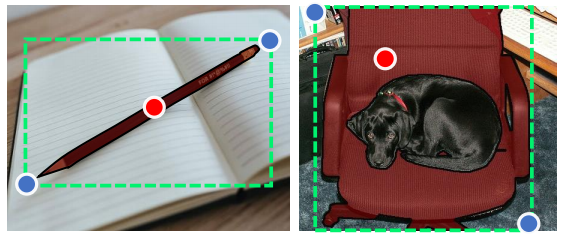
\includegraphics[width=\linewidth]{IoG}
\caption{Ukážka použitia prístupu \textit{Inside-Outside Guidance} pre užívateľský vstup. Prevzaté z \cite{zhang_liew_wei_wei_zhao_2020}.}
\end{figure}

Pri trénovaní siete nie je reálné, aby bol vstup získaný od skutočného užívateľa, ale musí byť náhodne vzorkovaný. Toto je implementované výberom bounding boxu z anotácie obrázku, ku ktorému je pripočítaný náhodný šum, aby vstup vyzeral ako od skutočného užívateľa. Kliknutie vo vnútri objektu je náhodne vygenerované vo vnútri objektu, s paddingom od okraja bounding boxu. Najväčšou výhodou tohto prístupu je schopnosť generalizovať aj iný typ predtým nevidených obrázkov bez potreby finetunovania.  

\section{Dataset}
Momentálne existujú mnohé dostupné datasety určené pre segmentáciu obrazu, ktoré sa dajú adaptovať aj na interaktívnu segmentáciu. Medzi najčastešie používané patrí \textit{Pascal}, \textit{Grabcut}, \textit{Berkley} alebo \textit{MS Coco}; a sú najčastejšie používané pre validáciu a porovnanie presnosti medzi dnešnými state-of-the-art systémami.

Pre náš projekt sme sa rozhodli použiť dataset \textit{MS Coco} pre evaluáciu aj trénovanie, pretože obsahuje cez 80 objektov vo viac ako 200 000 obrázkoch, ktoré zachytávajú bežné objekty zo života.

\begin{figure}[H]
\centering
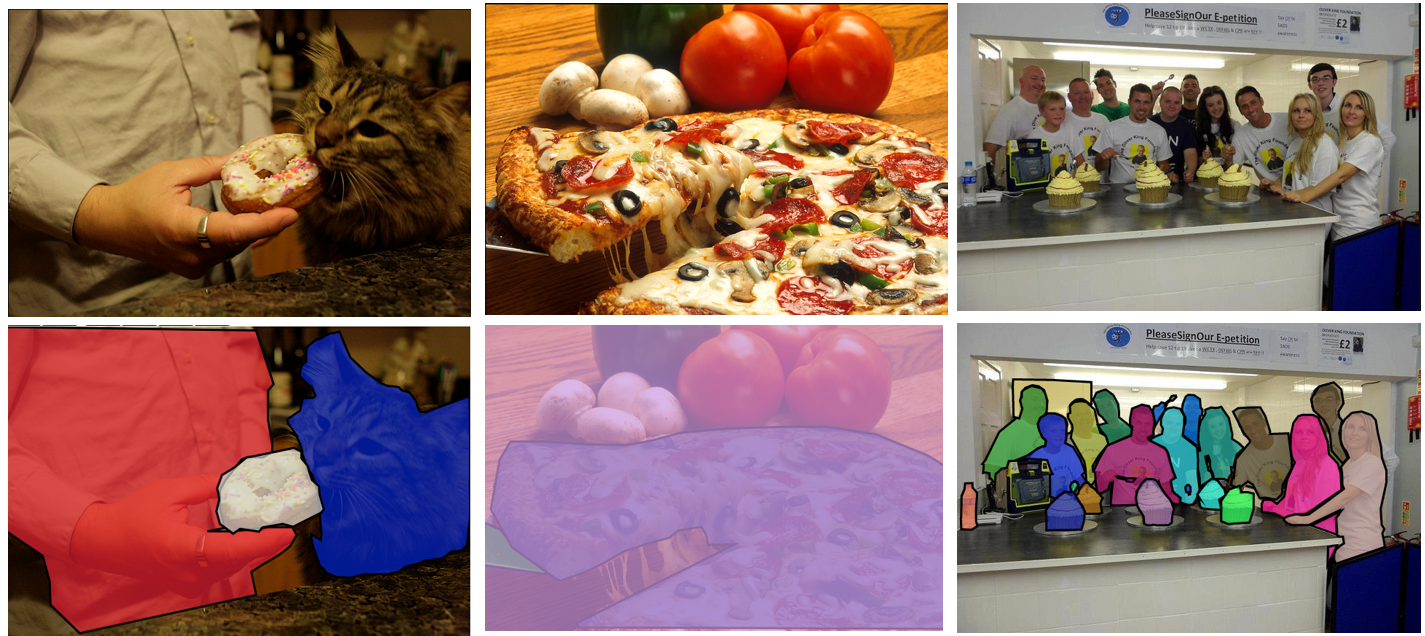
\includegraphics[width=\linewidth]{coco}
\caption{Ukážka obrázkov z datasetu \textit{MS Coco}. \\Prevzaté z \cite{coco}.}
\end{figure}

\section{Model}

Model pre túto úlohu je založený na dvoch podsieťach: \textit{CoarseNet} a \textit{FineNet}. Takáto architektúra bola pôvodne navrhnutá pre odhadnutie pózy človeka v obrázku. 

\begin{figure}[H]
\centering
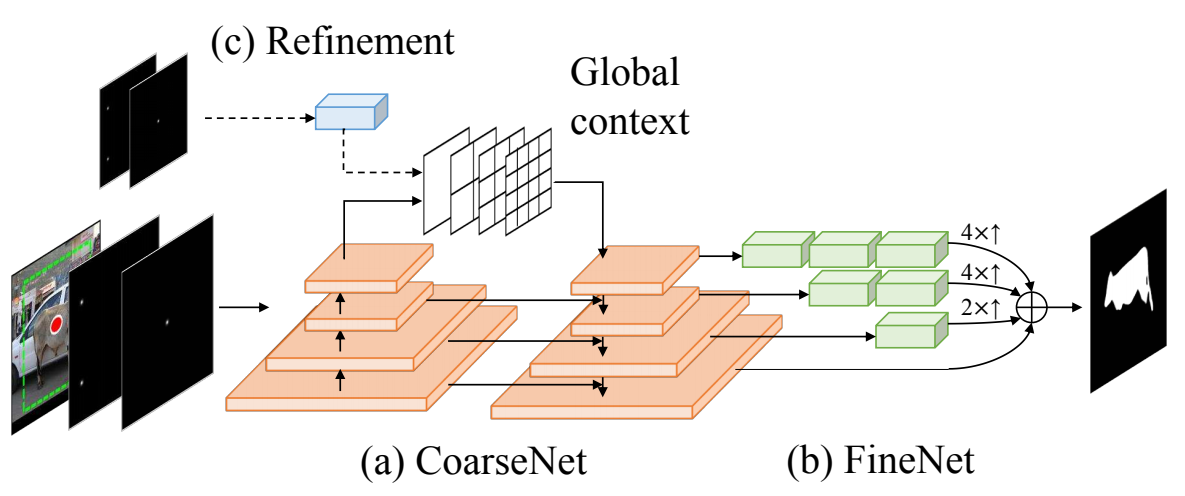
\includegraphics[width=\linewidth]{architecture}
\caption{Ukážka konceptu architektúry pre tento typ úlohy. Prevzaté z \cite{zhang_liew_wei_wei_zhao_2020}.}
\end{figure}


\textit{CoarseNet} má v našom prípade upravenú architektúru veľmi podobnú \textit{Resnet-50}, usporiadanej do pyramídovej štruktúry. Takáto sieť postupne aplikuje konvolúcie na vstupný batch obrázkov, na najhlbšej vrstve môže pridať \textit{refinement heatmapu} pre globálny kontext. Následne na najhlbšej vrstve aplikuje dekonvolúciu, až kým sa nedostane na pôvodnú veľkosť batchu obrázku. Ako aktivačná funkcia pre všetky vrstvy je použitá ReLU.

\textit{FineNet} je použitá na upsamplovanie medzivrstiev \textit{CoarseNetu}, ktoré sú následne skonkatenované a tvoria výstupný obrázok. Jej cieľom je obnoviť chýbajúce detaily, ako napríklad hranice objektu. \textit{FineNet} taktiež využíva ReLU na všetkých vrstvách okrem poslednej, kde je kvôli tresholdovaniu použitá sigmoida.

Pri trénovaní bol použitý learning rate s hodnotou $0.001$, optimalizátorom \textit{Adam} a chybová funkcia pre binárnu cross-entropiu.

\begin{figure}[H]
\centering
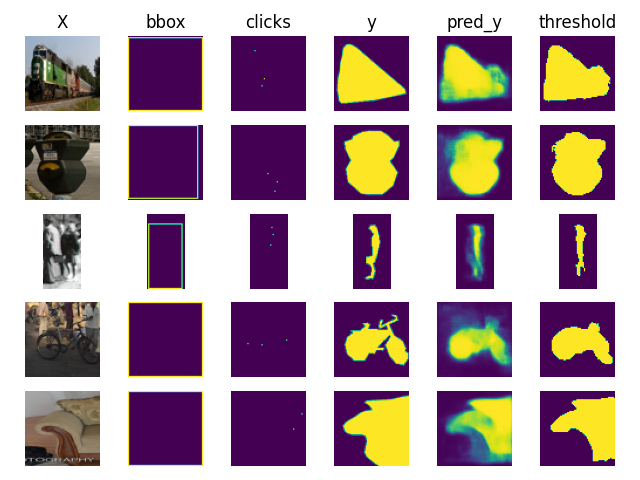
\includegraphics[width=\linewidth]{results}
\caption{Ukážka výsledkov z natrénovaného modelu. Zľava: originálny obrázok, použitý bounding box, použité kliknutia, očakávaná segmentácia objektu, predikcia modelu bez thresholdovania, predikcia modelu s thresholdovaním}
\end{figure}

\section{Evaluácia}
Po každej epoche trénovania bol model evaluovaný na základe 3 metrík (\cite{tiu_2020}):

\begin{itemize}
\item \textit{Pixel accuracy} - porovnáva, či sa jednotlivé pixely rovnajú; avšak táto metrika môže byť zavádzajúca, ak sú triedy na obrázku v nerovnováhe
\item \textit{Intersection over union (IoU)} - metrika, ktorá delí prienik očakávaného obrázku a predikcie modelu s ich zjednotením; najčastejšie používaná metrika pre porovnanie systémov
\item \textit{Dice coefficient} - metrika, ktorá používa dvojnásobok prieniku očakávaného obrázku a predikcie modelu podelený plochou oboch obrázkov v pixeloch 
\end{itemize}
Experimentálne boli implementované všetky 3 metriky, avšak pre výber najlepšieho modelu bola použitá metrika IoU, keďže väčšina systémov používa práve túto metriku pre prezentáciu výsledkov.

\section{Praktická aplikácia a GUI}

\bibliographystyle{czechiso}
\renewcommand{\refname}{Použitá literatúra}
\bibliography{bibliography}

\end{document}